\documentclass{article}
\usepackage[utf8]{inputenc}
\usepackage{hyperref}
\usepackage{graphicx}
\usepackage{fixltx2e}
\usepackage{bm}
\setlength{\parskip}{1em}
\usepackage[margin=1.0in]{geometry}
\usepackage{pgfplots}
\usepackage{subfig}
\usepackage{amsmath}
\usepackage[
    backend=bibtex, 
    natbib=true,
    style=numeric,
    sorting=none
    ]{biblatex}
\addbibresource{ref.bib}
\pgfplotsset{width=10cm,compat=1.9}
\usepgfplotslibrary{external}
\tikzexternalize

\title{Lab 4: Weight Training: A Numerical Example\\
  \large ECSE 421: Embedded Systems \\ Department of Electrical and Computer Engineering \\ McGill University \\ Version 1.1}
\author{Adam Cavatassi}
\date{Winter 2018}

\begin{document}

\maketitle

This document demonstrates a numerical example of one training iteration of the neural network example in the Lab 4 instructions. Recall the hypothetical neural network in Fig. \ref{fig:bp_ex}. This network has 2 inputs, a hidden layer with 2 nodes, and an output layer with 2 nodes. The hidden and output layer both use the sigmoid function as an activation. The network is to be trained using the mean squared error cost function. This example will utilize stochastic gradient descent with a batch size of 1 and a learning rate $\alpha = 0.1$. All numbers in this example were selected at random. Lets say that hypothetically, the batch for this iteration of training has the following input and target data:

\begin{equation}
\begin{matrix}
    \mathbf{i} = \bigg[\begin{matrix} 0.25 \\ -0.31 \end{matrix}\bigg] &
    \mathbf{t} = \bigg[\begin{matrix} 1 \\ 0 \end{matrix}\bigg]
\end{matrix}
\end{equation}

Your two weight matrices are initialized at random such that $\mathbf{W_k} \in \textit{U}[-1,1]$:

\begin{equation}
\begin{matrix}
    \mathbf{W_0} = \bigg[\begin{matrix} 0.81 & -0.03 \\ -0.63 & -0.21 \end{matrix}\bigg] &
    \mathbf{W_1} = \bigg[\begin{matrix} -0.76 & 0.55 \\ 0.21 & -0.11 \end{matrix}\bigg]
\end{matrix}
\end{equation}

We are now ready to complete a full iteration of training.

\begin{figure}[h!]
\centering
\hspace{3cm} 
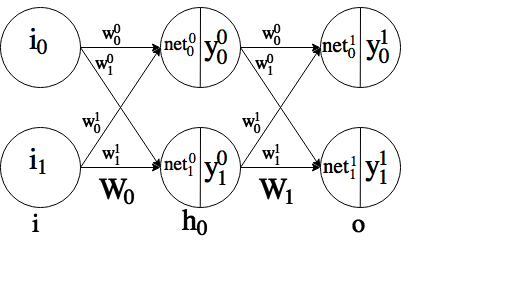
\includegraphics[scale=0.7]{figs/bp_ex.png}
\caption{Example neural network.}
\label{fig:bp_ex}
\end{figure}

\section*{Forward pass:}

First we need to compute the dot product for the hidden nodes:

\begin{equation}
    \mathbf{net^0} = \bigg[\begin{matrix} net_0^0 \\ net_1^0 \end{matrix}\bigg] =
    \bigg[\begin{matrix} i_0 w_0^0 + i_1 w_0^1 \\ i_0 w_1^0 + i_1 w_1^1 \end{matrix}\bigg] = 
    \bigg[\begin{matrix} (0.25)(0.81) + (-0.31)(-0.63) \\ (0.25)(-0.03) + (-0.31)(-0.21) \end{matrix}\bigg] =
    \bigg[\begin{matrix} 0.3978 \\ 0.0576 \end{matrix}\bigg]
\end{equation}

Next, we compute the activations for the hidden nodes:

\begin{equation}
    \mathbf{y^0} =
    \bigg[\begin{matrix} y_0^0 \\ y_1^0 \end{matrix}\bigg] = \bigg[\begin{matrix} \sigma(net_0^0) \\ \sigma(net_1^0) \end{matrix}\bigg] = 
    \bigg[\begin{matrix} \sigma(0.3978) \\ \sigma(0.0576) \end{matrix}\bigg] =
    \bigg[\begin{matrix} 0.5982 \\ 0.5144 \end{matrix}\bigg]
\end{equation}

Proceed to compute the dot product for the output layer:

\begin{equation}
    \mathbf{net^1} = \bigg[\begin{matrix} net_0^1 \\ net_1^1 \end{matrix}\bigg] =
    \bigg[\begin{matrix} y_0^0 w_0^0 + y_1^0 w_0^1 \\ y_0^0 w_1^0 + y_1^0 w_1^1 \end{matrix}\bigg] = 
    \bigg[\begin{matrix} (0.5982)(-0.76) + (0.5144)(0.21) \\ (0.5982)(0.55) + (0.5144)(-0.11) \end{matrix}\bigg] =
    \bigg[\begin{matrix} -0.3466 \\ 0.2724 \end{matrix}\bigg]
\end{equation}

Finally, compute the activation for the output layer:

\begin{equation}
    \mathbf{y^1} = \bigg[\begin{matrix} y_0^1 \\ y_1^1 \end{matrix}\bigg] =
    \bigg[\begin{matrix} \sigma(net_0^1) \\ \sigma(net_1^1) \end{matrix}\bigg] = 
    \bigg[\begin{matrix} \sigma(-0.3466 ) \\ \sigma(0.2724 \end{matrix}\bigg] =
    \bigg[\begin{matrix} 0.4142 \\ 0.5677 \end{matrix}\bigg]
\end{equation}

The forward pass is now complete, and we can move on to the backward pass.

\section*{Backward pass:}

Working backwards, we begin by computing the gradient for the output layer:

\begin{align*}
    \nabla J(\mathbf{W_1}) &= \mathbf{\boldsymbol{\delta}^1} \times \mathbf{y^0} \thinspace ^\top \\[0.5em]
    &= [(\mathbf{y^1}-\mathbf{t})\sigma(\mathbf{net^1})(1-\sigma(\mathbf{net^1})] \times \mathbf{y^0} \thinspace ^\top \\[0.5em]
    &= \Bigg[ \bigg(\bigg[\begin{matrix} 0.4142 \\ 0.5677 \end{matrix}\bigg] - \bigg[\begin{matrix} 1 \\ 0 \end{matrix}\bigg]\bigg)
    \sigma\bigg[\begin{matrix} -0.3466 \\ 0.2724 \end{matrix} \bigg]
    \bigg(1- \sigma\bigg[ \begin{matrix} -0.3466 \\ 0.2724 \end{matrix} \bigg] \bigg) \Bigg] \times 
    [ \begin{matrix} 0.5982 & 0.5144 \end{matrix} ] \\[0.5em]
    &= \bigg[\begin{matrix} -0.1421 \\ 0.1393 \end{matrix}\bigg] \times 
    [ \begin{matrix} 0.5982 & 0.0.5144 \end{matrix} ] \\[0.5em]
    &= \bigg[\begin{matrix} -0.085 & -0.0730 \\ 0.0833 & 0.0716 \end{matrix}\bigg]
\end{align*}


And then the gradient for the hidden layer:

\begin{align*}
    \nabla J(\mathbf{W_0}) &= \mathbf{\boldsymbol{\delta}^0} \times \mathbf{i} \thinspace ^\top \\[0.5em]
    &= [(\mathbf{W_1} \times \mathbf{\boldsymbol{\delta}^1}) \sigma(\mathbf{net^0})(1-\sigma(\mathbf{net^0})] \times \mathbf{i} \thinspace ^\top \\[0.5em]
    &= \Bigg[ \Bigg(\bigg[\begin{matrix} -0.76 & 0.55 \\ 0.21 & -0.11 \end{matrix}\bigg] \times \bigg[\begin{matrix} -0.1421 \\ 0.1393 \end{matrix} \bigg]\Bigg)
    \sigma\bigg[\begin{matrix} 0.3978\\ 0.0576 \end{matrix} \bigg]
    \bigg(1- \sigma\bigg[ \begin{matrix} 0.3978\\ 0.0576 \end{matrix} \bigg] \bigg) \Bigg] \times 
    [ \begin{matrix} 0.25 & -0.31 \end{matrix} ] \\[0.5em]
    &= \Bigg[ \bigg[\begin{matrix} 0.1846 \\ -0.0452  \end{matrix}\bigg]
              \bigg[\begin{matrix} 0.5982 \\ 0.5144  \end{matrix}\bigg]
              \bigg(1- \bigg[\begin{matrix} 0.5982 \\ 0.5144  \end{matrix}\bigg] \bigg) \Bigg] \times 
    [ \begin{matrix} 0.25 & -0.31 \end{matrix} ] \\[0.5em]
    &= \bigg[\begin{matrix} 0.0444 \\ -0.0113 \end{matrix}\bigg] \times 
    [ \begin{matrix} 0.25 & -0.31 \end{matrix} ] \\[0.5em]
    &= \bigg[\begin{matrix} 0.0111 & -0.0138 \\ -0.0028 & 0.0035 \end{matrix}\bigg]
\end{align*}

Now we can update the weights for both layers:

\begin{align*}
   \mathbf{W_0}_{new} &= \mathbf{W_0}_{old} - \alpha \nabla J(\mathbf{W_0}) \\[0.5em]
   &= \bigg[\begin{matrix} 0.81 & -0.03 \\ -0.63 & -0.21 \end{matrix}\bigg] - 0.1\bigg[\begin{matrix} 0.0111 & -0.0138 \\ -0.0028 & 0.0035 \end{matrix}\bigg] \\[0.5em]
   &= \bigg[\begin{matrix} 0.81 & -0.03 \\ -0.63 & -0.21 \end{matrix}\bigg] - \bigg[\begin{matrix} 0.00111 & -0.00138 \\ -0.00028 & 0.00035 \end{matrix}\bigg] \\[0.5em]
   &= \bigg[\begin{matrix} 0.80889 & -0.02862 \\ -0.62972 & -0.21035 \end{matrix}\bigg]
\end{align*}

\begin{align*}
   \mathbf{W_1}_{new} &= \mathbf{W_1}_{old} - \alpha \nabla J(\mathbf{W_1}) \\[0.5em]
   &= \bigg[\begin{matrix} -0.76 & 0.55 \\ 0.21 & -0.11 \end{matrix}\bigg] - 0.1\bigg[\begin{matrix} -0.085 & -0.0730 \\ 0.0833 & 0.0716 \end{matrix}\bigg] \\[0.5em]
   &= \bigg[\begin{matrix} -0.76 & 0.55 \\ 0.21 & -0.11 \end{matrix}\bigg] - \bigg[\begin{matrix} -0.0085 & -0.00730 \\ 0.00833 & 0.00716 \end{matrix}\bigg] \\[0.5em]
   &= \bigg[\begin{matrix} 0.7515 & -0.0.5573\\ 0.20167 & -0.11716 \end{matrix}\bigg]
\end{align*}

We have now completed one full training iteration. This process must be repeated until the training and validation error are sufficiently low. 

\end{document}